\newpage
\subsection{Caso d'uso UC12: Gestione proprio profilo utente}
\label{UC12}
\begin{figure}[ht]
	\centering
	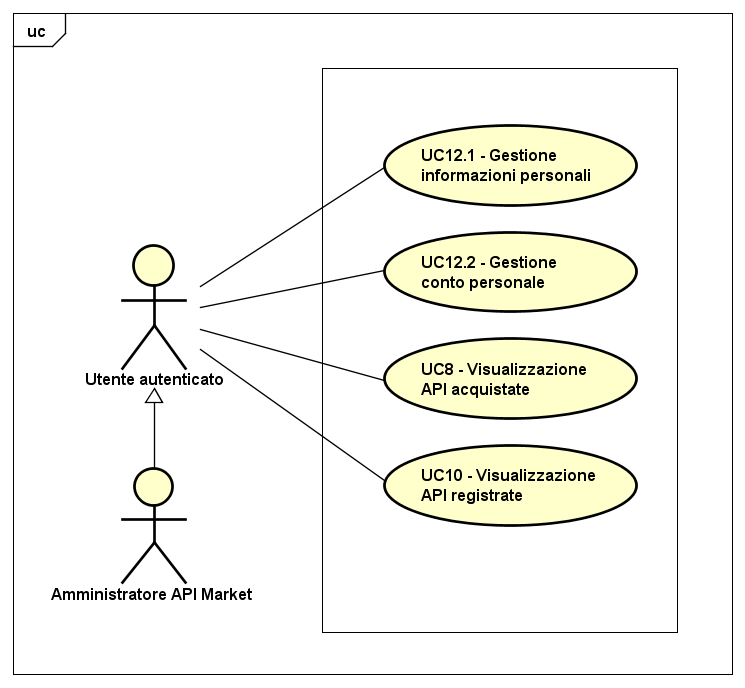
\includegraphics[scale=0.45]{UML/UC12.png}
	\caption{UC12 - Gestione proprio profilo utente}
\end{figure}

\begin{longtable}{ l | p{11cm}}
	\hline
	\rowcolor{Gray}
	\multicolumn{2}{c}{UC12 - Gestione proprio profilo utente} \\
	\hline
	\textbf{Attori} & Utente autenticato, Amministratore API Market \\
	\textbf{Descrizione} & L'attore visualizza e/o gestisce le informazioni del proprio profilo utente \\
	\textbf{Pre-Condizioni} & L'attore si trova nella schermata relativa alla gestione del proprio profilo utente \\
	\textbf{Post-Condizioni} & L'attore ha visualizzato e/o gestito le informazioni del proprio profilo utente \\
	\textbf{Scenario Principale} & 
	\begin{enumerate*}[label=(\arabic*.),itemjoin={\newline}]
		\item L'attore può gestire le proprie informazioni personali (UC12.1)
		\item L'attore può gestire il proprio conto utente (UC12.2)
		\item L'attore può visualizzare le API da lui acquistate (UC8)
		\item L'attore può visualizzare le API da lui registrate (UC10)
	\end{enumerate*}\\
\end{longtable}

\newpage
\subsubsection{Caso d'uso UC12.1: Gestione informazioni personali}
\label{UC12_1}
\begin{figure}[ht]
	\centering
	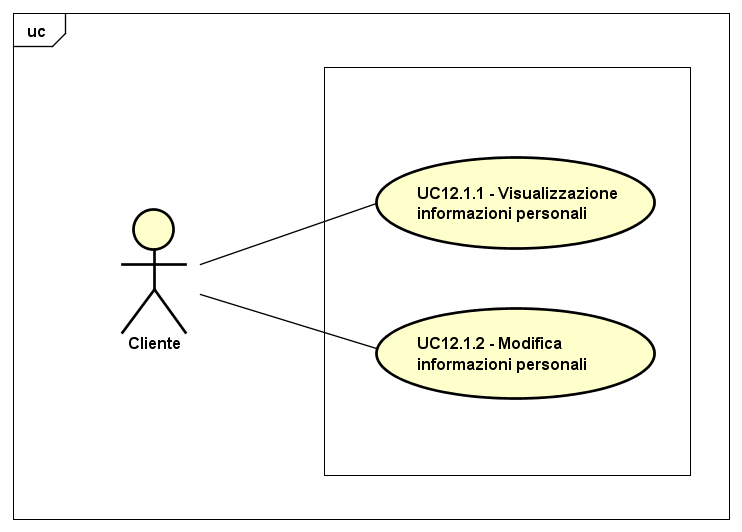
\includegraphics[scale=0.45]{UML/UC12_1.png}
	\caption{UC12.1: Gestione informazioni personali}
\end{figure}

\begin{minipage}{\linewidth}
	\begin{tabular}{ l | p{11cm}}
		\hline
		\rowcolor{Gray}
		\multicolumn{2}{c}{UC12.1 - Gestione informazioni personali} \\
		\hline
		\textbf{Attori} & Utente autenticato, Amministratore API Market \\
		\textbf{Descrizione} & L'attore visualizza e/o modifica le proprie informazioni personali \\
		\textbf{Pre-Condizioni} & L'attore si trova nella schermata relativa alla gestione del proprio profilo utente \\
		\textbf{Post-Condizioni} & L'attore ha visualizzato e/o modificato le proprie informazioni personali \\
		\textbf{Scenario Principale} & 
		\begin{enumerate*}[label=(\arabic*.),itemjoin={\newline}]
			\item L'attore può visualizzare le proprie informazioni personali (UC12.1.1)
			\item L'attore può modificare le proprie informazioni personali (UC12.1.2)
		\end{enumerate*}
	\end{tabular}
\end{minipage}

\newpage
\paragraph{Caso d'uso UC12.1.1: Visualizzazione informazioni personali}
\label{UC12_1_1}
\begin{figure}[ht]
	\centering
	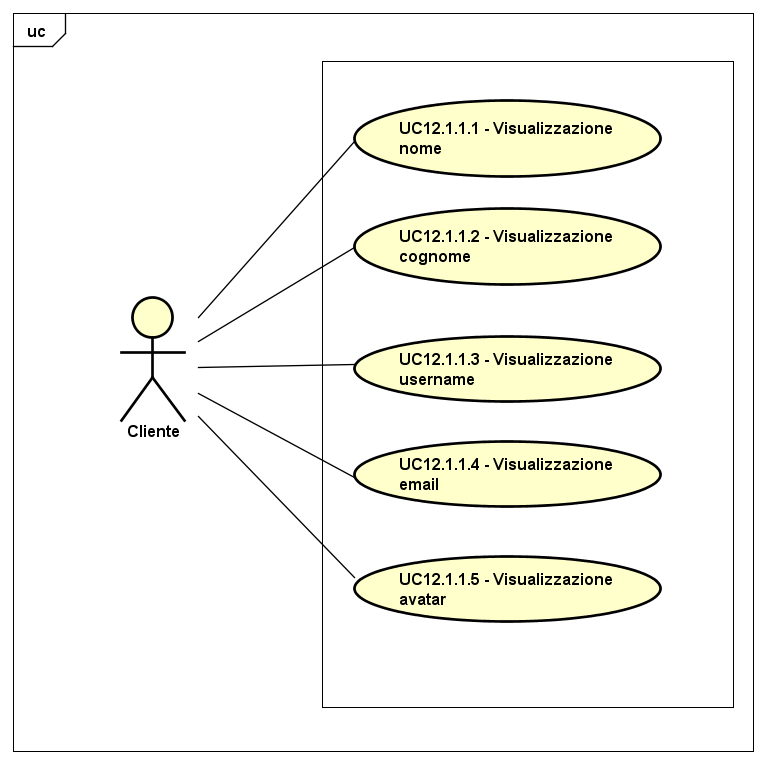
\includegraphics[scale=0.45]{UML/UC12_1_1.png}
	\caption{UC12.1.1: Visualizzazione informazioni personali}
\end{figure}

\begin{minipage}{\linewidth}
\begin{tabular}{ l | p{11cm}}
	\hline
	\rowcolor{Gray}
	\multicolumn{2}{c}{UC12.1.1 - Visualizzazione informazioni personali} \\
	\hline
	\textbf{Attori} & Utente autenticato, Amministratore API Market \\
	\textbf{Descrizione} & L'attore visualizza le proprie informazioni personali \\
	\textbf{Pre-Condizioni} & L'attore si trova nella schermata relativa alla gestione del proprio profilo utente \\
	\textbf{Post-Condizioni} & L'attore ha visualizzato le proprie informazioni personali \\
	\textbf{Scenario Principale} & 
	\begin{enumerate*}[label=(\arabic*.),itemjoin={\newline}]
		\item L'attore può visualizzare il proprio nome (UC12.1.1.1)
		\item L'attore può visualizzare il proprio cognome (UC12.1.1.2)
		\item L'attore può visualizzare il proprio username (UC12.1.1.3)
		\item L'attore può visualizzare la propria email (UC12.1.1.4)
		\item L'attore può visualizzare il proprio avatar (UC12.1.1.5)
	\end{enumerate*}\\
\end{tabular}
\end{minipage}

\subparagraph{Caso d'uso UC12.1.1.1: Visualizzazione nome}
\label{UC12_1_1_1}

\begin{minipage}{\linewidth}
\begin{tabular}{ l | p{11cm}}
	\hline
	\rowcolor{Gray}
	\multicolumn{2}{c}{UC12.1.1.1 - Visualizzazione nome} \\
	\hline
	\textbf{Attori} & Utente autenticato, Amministratore API Market \\
	\textbf{Descrizione} & L'attore visualizzare il proprio nome \\
	\textbf{Pre-Condizioni} & L'attore si trova nella schermata relativa alla gestione delle informazioni personali \\
	\textbf{Post-Condizioni} & L'attore ha visualizzato il proprio nome \\
	\textbf{Scenario Principale} & 
	\begin{enumerate*}[label=(\arabic*.),itemjoin={\newline}]
		\item L'attore può visualizzare il proprio nome
	\end{enumerate*}
\end{tabular}
\end{minipage}

\subparagraph{Caso d'uso UC12.1.1.2: Visualizzazione cognome}
\label{UC12_1_1_2}

\begin{minipage}{\linewidth}
	\begin{tabular}{ l | p{11cm}}
		\hline
		\rowcolor{Gray}
		\multicolumn{2}{c}{UC12.1.1.2 - Visualizzazione cognome} \\
		\hline
		\textbf{Attori} & Utente autenticato, Amministratore API Market \\
		\textbf{Descrizione} & L'attore visualizzare il proprio cognome \\
	\textbf{Pre-Condizioni} & L'attore si trova nella schermata relativa alla gestione delle informazioni personali \\
	\textbf{Post-Condizioni} & L'attore ha visualizzato il proprio cognome \\
	\textbf{Scenario Principale} & 
	\begin{enumerate*}[label=(\arabic*.),itemjoin={\newline}]
		\item L'attore può visualizzare il proprio cognome
	\end{enumerate*}
	\end{tabular}
\end{minipage}

\subparagraph{Caso d'uso UC12.1.1.3: Visualizzazione username}
\label{UC12_1_1_3}

\begin{minipage}{\linewidth}
	\begin{tabular}{ l | p{11cm}}
		\hline
		\rowcolor{Gray}
		\multicolumn{2}{c}{UC12.1.1.3 - Visualizzazione username} \\
		\hline
		\textbf{Descrizione} & L'attore visualizzare il proprio username \\
	\textbf{Pre-Condizioni} & L'attore si trova nella schermata relativa alla gestione delle informazioni personali \\
	\textbf{Post-Condizioni} & L'attore ha visualizzato il proprio username \\
	\textbf{Scenario Principale} & 
	\begin{enumerate*}[label=(\arabic*.),itemjoin={\newline}]
		\item L'attore può visualizzare il proprio username
	\end{enumerate*}
	\end{tabular}
\end{minipage}

\subparagraph{Caso d'uso UC12.1.1.4: Visualizzazione email}
\label{UC12_1_1_4}

\begin{minipage}{\linewidth}
	\begin{tabular}{ l | p{11cm}}
		\hline
		\rowcolor{Gray}
		\multicolumn{2}{c}{UC12.1.1.4 - Visualizzazione email} \\
		\hline
		\textbf{Attori} & Utente autenticato, Amministratore API Market \\
		\textbf{Descrizione} & L'attore visualizzare la propria email \\
		\textbf{Pre-Condizioni} & L'attore si trova nella schermata relativa alla gestione delle informazioni personali \\
		\textbf{Post-Condizioni} & L'attore ha visualizzato la propria email \\
		\textbf{Scenario Principale} & 
		\begin{enumerate*}[label=(\arabic*.),itemjoin={\newline}]
			\item L'attore può visualizzare la propria email
		\end{enumerate*}
	\end{tabular}
\end{minipage}

\subparagraph{Caso d'uso UC12.1.1.5: Visualizzazione avatar}
\label{UC12_1_1_5}

\begin{minipage}{\linewidth}
	\begin{tabular}{ l | p{11cm}}
		\hline
		\rowcolor{Gray}
		\multicolumn{2}{c}{UC12.1.1.5 - Visualizzazione avatar} \\
		\hline
		\textbf{Attori} & Utente autenticato, Amministratore API Market \\
		\textbf{Descrizione} & L'attore visualizzare il proprio avatar \\
		\textbf{Pre-Condizioni} & L'attore si trova nella schermata relativa alla gestione delle informazioni personali \\
		\textbf{Post-Condizioni} & L'attore ha visualizzato il proprio avatar \\
		\textbf{Scenario Principale} & 
		\begin{enumerate*}[label=(\arabic*.),itemjoin={\newline}]
			\item L'attore può visualizzare il proprio avatar
		\end{enumerate*}
	\end{tabular}
\end{minipage}

\newpage
\paragraph{Caso d'uso UC12.1.2: Modifica informazioni personali}
\label{UC12_1_2}
\begin{figure}[ht]
	\centering
	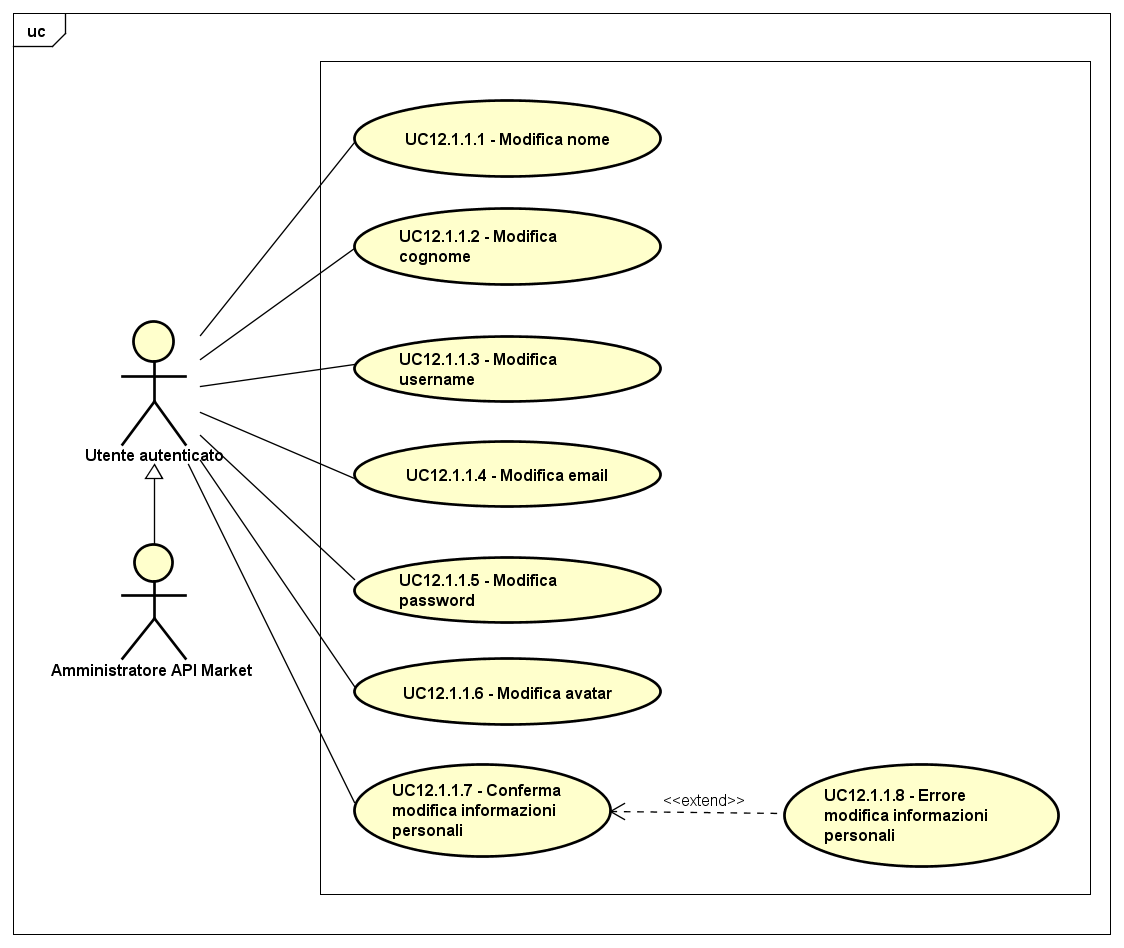
\includegraphics[scale=0.45]{UML/UC12_1_2.png}
	\caption{UC12.1.2: Modifica informazioni personali}
\end{figure}

\begin{tabular}{ l | p{11cm}}
	\hline
	\rowcolor{Gray}
	\multicolumn{2}{c}{UC12.1.2 - Modifica informazioni personali} \\
	\hline
	\textbf{Attori} & Utente autenticato, Amministratore API Market \\
	\textbf{Descrizione} & L'attore modifica le proprie informazioni personali \\
	\textbf{Pre-Condizioni} & L'attore si trova nella schermata relativa alla gestione del proprio profilo utente \\
	\textbf{Post-Condizioni} & L'attore ha modificato le proprie informazioni personali \\
	\textbf{Scenario Principale} & 
	\begin{enumerate*}[label=(\arabic*.),itemjoin={\newline}]
		\item L'attore può modificare il proprio nome (UC12.1.2.1)
		\item L'attore può modificare il proprio cognome (UC12.1.2.2)
		\item L'attore può modificare il proprio username (UC12.1.2.3)
		\item L'attore può modificare la propria email (UC12.1.2.4)
		\item L'attore può modificare la propria password (UC12.1.2.5)
		\item L'attore può modificare il proprio avatar (UC12.1.2.6)
		\item L'attore può confermare la modifica alle proprie informazione personali (UC12.1.2.7)
	\end{enumerate*}\\
	\textbf{Scenari Alternativi} & 
	\begin{enumerate*}[label=(\arabic*.),itemjoin={\newline}]
		\item L'attore può visualizzare un messaggio di errore informativo, e le modifiche non avvengono (UC12.1.2.8)
	\end{enumerate*}\\
\end{tabular}

\subparagraph{Caso d'uso UC12.1.2.1: Modifica nome}
\label{UC12_1_2_1}

\begin{minipage}{\linewidth}
	\begin{tabular}{ l | p{11cm}}
		\hline
		\rowcolor{Gray}
		\multicolumn{2}{c}{UC12.1.2.1 - Modifica nome} \\
		\hline
		\textbf{Attori} & Utente autenticato, Amministratore API Market \\
		\textbf{Descrizione} & L'attore modifica il proprio nome \\
		\textbf{Pre-Condizioni} & L'attore si trova nella schermata relativa alla gestione delle informazioni personali \\
		\textbf{Post-Condizioni} & L'attore ha modificato il proprio nome \\
		\textbf{Scenario Principale} & 
		\begin{enumerate*}[label=(\arabic*.),itemjoin={\newline}]
			\item L'attore può modificare il proprio nome
		\end{enumerate*}
	\end{tabular}
\end{minipage}

\subparagraph{Caso d'uso UC12.1.2.2: Modifica cognome}
\label{UC12_1_2_2}

\begin{minipage}{\linewidth}
	\begin{tabular}{ l | p{11cm}}
		\hline
		\rowcolor{Gray}
		\multicolumn{2}{c}{UC12.1.2.2 - Modifica cognome} \\
		\hline
		\textbf{Attori} & Utente autenticato, Amministratore API Market \\
		\textbf{Descrizione} & L'attore modifica il proprio cognome \\
		\textbf{Pre-Condizioni} & L'attore si trova nella schermata relativa alla gestione delle informazioni personali \\
		\textbf{Post-Condizioni} & L'attore ha modificato il proprio cognome \\
		\textbf{Scenario Principale} & 
		\begin{enumerate*}[label=(\arabic*.),itemjoin={\newline}]
			\item L'attore può modificare il proprio cognome
		\end{enumerate*}
	\end{tabular}
\end{minipage}

\subparagraph{Caso d'uso UC12.1.2.3: Modifica username}
\label{UC12_1_2_3}

\begin{minipage}{\linewidth}
	\begin{tabular}{ l | p{11cm}}
		\hline
		\rowcolor{Gray}
		\multicolumn{2}{c}{UC12.1.2.3 - Modifica username} \\
		\hline
		\textbf{Attori} & Utente autenticato, Amministratore API Market \\
		\textbf{Descrizione} & L'attore modifica il proprio username \\
		\textbf{Pre-Condizioni} & L'attore si trova nella schermata relativa alla gestione delle informazioni personali \\
		\textbf{Post-Condizioni} & L'attore ha modificato il proprio username \\
		\textbf{Scenario Principale} & 
		\begin{enumerate*}[label=(\arabic*.),itemjoin={\newline}]
			\item L'attore può modificare il proprio username
		\end{enumerate*}
	\end{tabular}
\end{minipage}

\subparagraph{Caso d'uso UC12.1.2.4: Modifica email}
\label{UC12_1_2_4}

\begin{minipage}{\linewidth}
	\begin{tabular}{ l | p{11cm}}
		\hline
		\rowcolor{Gray}
		\multicolumn{2}{c}{UC12.1.2.4 - Modifica email} \\
		\hline
		\textbf{Attori} & Utente autenticato, Amministratore API Market \\
		\textbf{Descrizione} & L'attore modifica la propria email \\
		\textbf{Pre-Condizioni} & L'attore si trova nella schermata relativa alla gestione delle informazioni personali \\
		\textbf{Post-Condizioni} & L'attore ha modificato la propria email \\
		\textbf{Scenario Principale} & 
		\begin{enumerate*}[label=(\arabic*.),itemjoin={\newline}]
			\item L'attore può modificare la propria email
		\end{enumerate*}
	\end{tabular}
\end{minipage}

\subparagraph{Caso d'uso UC12.1.2.5: Modifica password}
\label{UC12_1_2_5}

\begin{minipage}{\linewidth}
	\begin{tabular}{ l | p{11cm}}
		\hline
		\rowcolor{Gray}
		\multicolumn{2}{c}{UC12.1.2.5 - Modifica password} \\
		\hline
		\textbf{Attori} & Utente autenticato, Amministratore API Market \\
		\textbf{Descrizione} & L'attore modifica la propria password \\
		\textbf{Pre-Condizioni} & L'attore si trova nella schermata relativa alla gestione delle informazioni personali \\
		\textbf{Post-Condizioni} & L'attore ha modificato la propria password \\
		\textbf{Scenario Principale} & 
		\begin{enumerate*}[label=(\arabic*.),itemjoin={\newline}]
			\item L'attore può modificare la propria password
		\end{enumerate*}
	\end{tabular}
\end{minipage}

\subparagraph{Caso d'uso UC12.1.2.6: Modifica avatar}
\label{UC12_1_2_6}

\begin{minipage}{\linewidth}
	\begin{tabular}{ l | p{11cm}}
		\hline
		\rowcolor{Gray}
		\multicolumn{2}{c}{UC12.1.2.6 - Modifica avatar} \\
		\hline
		\textbf{Attori} & Utente autenticato, Amministratore API Market \\
		\textbf{Descrizione} & L'attore modifica il proprio avatar \\
		\textbf{Pre-Condizioni} & L'attore si trova nella schermata relativa alla gestione delle informazioni personali \\
		\textbf{Post-Condizioni} & L'attore ha modificato il proprio avatar \\
		\textbf{Scenario Principale} & 
		\begin{enumerate*}[label=(\arabic*.),itemjoin={\newline}]
			\item L'attore può modificare il proprio avatar
		\end{enumerate*}
	\end{tabular}
\end{minipage}

\subparagraph{Caso d'uso UC12.1.2.7: Conferma modifica informazioni personali}
\label{UC12_1_2_7}

\begin{minipage}{\linewidth}
	\begin{tabular}{ l | p{11cm}}
		\hline
		\rowcolor{Gray}
		\multicolumn{2}{c}{UC12.1.2.7 - Conferma modifica informazioni personali} \\
		\hline
		\textbf{Attori} & Utente autenticato, Amministratore API Market \\
		\textbf{Descrizione} & L'attore conferma la modifica delle informazioni personali \\
		\textbf{Pre-Condizioni} & L'attore si trova nella schermata relativa alla gestione delle informazioni personali \\
		\textbf{Post-Condizioni} & L'attore ha confermato la modifica delle informazioni personali \\
		\textbf{Scenario Principale} & 
		\begin{enumerate*}[label=(\arabic*.),itemjoin={\newline}]
			\item L'attore può confermare la modifica delle informazioni personali, visualizzando un messaggio di successo
		\end{enumerate*}\\
	\end{tabular}
\end{minipage}

\subparagraph{Caso d'uso UC12.1.2.8: Errore modifica informazioni personali}
\label{UC12_1_2_8}

\begin{minipage}{\linewidth}
	\begin{tabular}{ l | p{11cm}}
		\hline
		\rowcolor{Gray}
		\multicolumn{2}{c}{UC12.1.2.8 - Errore modifica informazioni personali} \\
		\hline
		\textbf{Attori} & Utente autenticato, Amministratore API Market \\
		\textbf{Descrizione} & L'attore visualizza un messaggio di errore informativo e la modifica delle informazioni personali non avviene \\
		\textbf{Pre-Condizioni} & L'attore ha confermato la modifica delle informazioni personali ma si è verificato un errore \\
		\textbf{Post-Condizioni} & L'attore ha visualizzato un messaggio di errore informativo \\
		\textbf{Scenario Principale} & 
		\begin{enumerate*}[label=(\arabic*.),itemjoin={\newline}]
			\item L'attore può visualizzare un messaggio di errore informativo e la modifica delle informazioni personali non avviene
		\end{enumerate*}\\
	\end{tabular}
\end{minipage}

\newpage
\subsubsection{Caso d'uso UC12.2: Gestione conto personale}
\label{UC12_2}
\begin{figure}[ht]
	\centering
	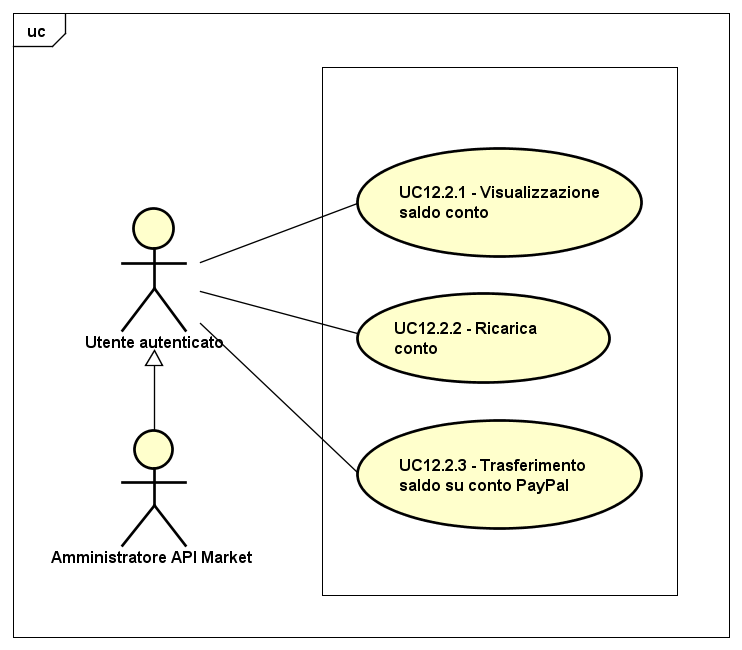
\includegraphics[scale=0.45]{UML/UC12_2.png}
	\caption{UC12.2: Gestione conto personale}
\end{figure}

\begin{minipage}{\linewidth}
	\begin{tabular}{ l | p{11cm}}
		\hline
		\rowcolor{Gray}
		\multicolumn{2}{c}{UC12.2 - Gestione conto personale} \\
		\hline
		\textbf{Attori} & Utente autenticato, Amministratore API Market \\
		\textbf{Descrizione} & L'attore visualizza le informazioni del proprio conto utente e/o effettua una ricarica su di esso \\
		\textbf{Pre-Condizioni} & L'attore si trova nella schermata relativa alla gestione del proprio profilo utente \\
		\textbf{Post-Condizioni} & L'attore ha visualizzato il saldo del proprio conto utente e/o effettuato una ricarica su di esso \\
		\textbf{Scenario Principale} & 
		\begin{enumerate*}[label=(\arabic*.),itemjoin={\newline}]
			\item L'attore può visualizzare il saldo corrente del proprio conto utente (UC12.2.1)
			\item L'attore può effettuare una ricarica sul proprio conto utente (UC12.2.2)
		\end{enumerate*}
	\end{tabular}
\end{minipage}

\paragraph{Caso d'uso UC12.2.1: Visualizzazione saldo conto}
\label{UC12_2_1}

\begin{minipage}{\linewidth}
	\begin{tabular}{ l | p{11cm}}
		\hline
		\rowcolor{Gray}
		\multicolumn{2}{c}{UC12.2.1 - Visualizzazione saldo conto} \\
		\hline
		\textbf{Attori} & Utente autenticato, Amministratore API Market \\
		\textbf{Descrizione} & L'attore visualizza il saldo corrente del proprio conto utente \\
		\textbf{Pre-Condizioni} & L'attore si trova nella schermata relativa alla gestione del proprio conto utente \\
		\textbf{Post-Condizioni} & L'attore ha visualizzato il saldo corrente del proprio conto utente \\
		\textbf{Scenario Principale} & 
		\begin{enumerate*}[label=(\arabic*.),itemjoin={\newline}]
			\item L'attore può visualizzare il saldo corrente del proprio conto utente
		\end{enumerate*}\\
	\end{tabular}
\end{minipage}

\paragraph{Caso d'uso UC12.2.2: Ricarica conto}
\label{UC12_2_2}
\begin{figure}[ht]
	\centering
	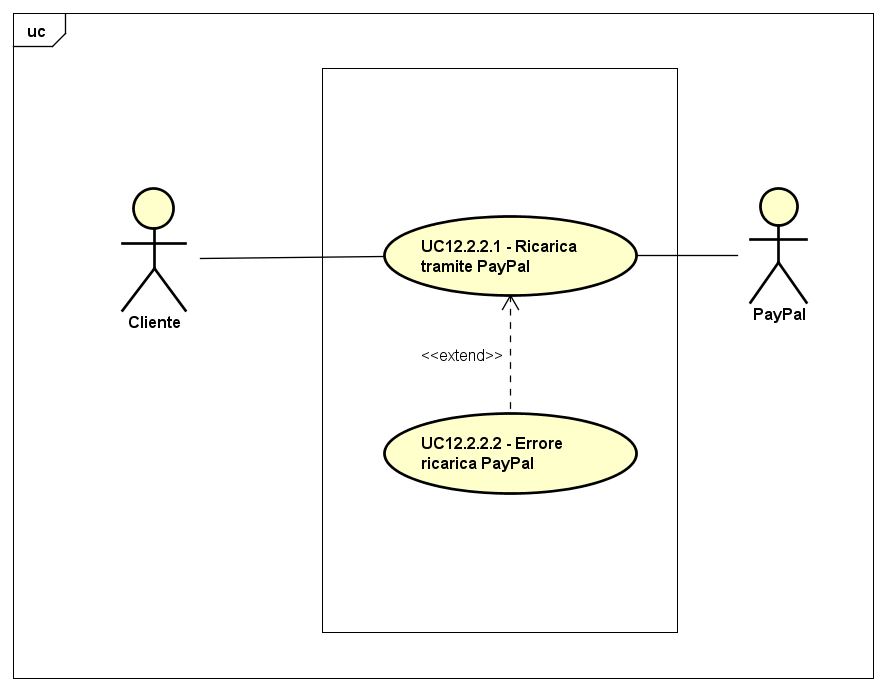
\includegraphics[scale=0.45]{UML/UC12_2_2.png}
	\caption{UC12.2.2: Ricarica conto}
\end{figure}

\begin{minipage}{\linewidth}
	\begin{tabular}{ l | p{11cm}}
		\hline
		\rowcolor{Gray}
		\multicolumn{2}{c}{UC12.2.2 - Ricarica conto} \\
		\hline
		\textbf{Attori} & Utente autenticato, Amministratore API Market, PayPal \\
		\textbf{Descrizione} & L'attore effettua una ricarica sul proprio conto utente \\
		\textbf{Pre-Condizioni} & L'attore si trova nella schermata relativa alla gestione del proprio conto utente \\
		\textbf{Post-Condizioni} & L'attore ha effettuato una ricarica sul proprio conto utente \\
		\textbf{Scenario Principale} & 
		\begin{enumerate*}[label=(\arabic*.),itemjoin={\newline}]
			\item L'attore può effettuare una ricarica tramite PayPal sul proprio conto utente (UC12.2.2.1)
		\end{enumerate*}\\
		\textbf{Scenari Alternativi} & \begin{enumerate*}[label=(\arabic*.),itemjoin={\newline}]
			\item L'attore può visualizzare un messaggio di errore informativo, e la ricarica tramite PayPal sul proprio conto utente non avviene (UC12.2.2.2)
		\end{enumerate*}\\
	\end{tabular}
\end{minipage}

\subparagraph{Caso d'uso UC12.2.2.1: Ricarica tramite PayPal}
\label{UC12_2_2_1}

\begin{minipage}{\linewidth}
	\begin{tabular}{ l | p{11cm}}
		\hline
		\rowcolor{Gray}
		\multicolumn{2}{c}{UC12.2.2.1 - Ricarica tramite PayPal} \\
		\hline
		\textbf{Attori} & Utente autenticato, Amministratore API Market, PayPal \\
		\textbf{Descrizione} & L'attore effettua una ricarica tramite PayPal sul proprio conto utente \\
		\textbf{Pre-Condizioni} & L'attore si trova nella schermata relativa alla ricarica del proprio conto utente \\
		\textbf{Post-Condizioni} & L'attore ha effettuato una ricarica tramite PayPal sul proprio conto utente \\
		\textbf{Scenario Principale} & 
		\begin{enumerate*}[label=(\arabic*.),itemjoin={\newline}]
			\item L'attore può effettuare una ricarica tramite PayPal sul proprio conto utente
		\end{enumerate*}\\
	\end{tabular}
\end{minipage}

\subparagraph{Caso d'uso UC12.2.2.2: Errore ricarica PayPal}
\label{UC12_2_2_2}

\begin{minipage}{\linewidth}
	\begin{tabular}{ l | p{11cm}}
		\hline
		\rowcolor{Gray}
		\multicolumn{2}{c}{UC12.2.2.2 - Errore ricarica PayPal} \\
		\hline
		\textbf{Attori} & Utente autenticato, Amministratore API Market, PayPal \\
		\textbf{Descrizione} & L'attore visualizza un messaggio di errore informativo e la ricarica tramite PayPal sul proprio conto utente non avviene \\
		\textbf{Pre-Condizioni} & L'attore ha confermato la ricarica tramite PayPal sul proprio conto utente ma si è verificato un errore \\
		\textbf{Post-Condizioni} & L'attore ha visualizzato un messaggio di errore informativo \\
		\textbf{Scenario Principale} & 
		\begin{enumerate*}[label=(\arabic*.),itemjoin={\newline}]
			\item L'attore può visualizzare un messaggio di errore informativo e la ricarica tramite PayPal sul proprio conto utente non avviene
		\end{enumerate*}\\
	\end{tabular}
\end{minipage}

\paragraph{Caso d'uso UC12.2.3: Trasferimento saldo su conto PayPal}
\label{UC12_2_3}

\begin{minipage}{\linewidth}
	\begin{tabular}{ l | p{11cm}}
		\hline
		\rowcolor{Gray}
		\multicolumn{2}{c}{UC12.2.3 - Trasferimento saldo su conto PayPal} \\
		\hline
		\textbf{Attori} & Utente autenticato, Amministratore API Market \\
		\textbf{Descrizione} & L'attore preleva una somma limitata di denaro dal proprio conto utente e la trasferisce su un conto PayPal \\
		\textbf{Pre-Condizioni} & L'attore si trova nella schermata relativa alla gestione del proprio conto utente \\
		\textbf{Post-Condizioni} & L'attore ha prelevato una somma limitata di denaro dal proprio conto utente e l'ha trasferita su un conto PayPal \\
		\textbf{Scenario Principale} & 
		\begin{enumerate*}[label=(\arabic*.),itemjoin={\newline}]
			\item L'attore può prelevare una somma limitata di denaro dal proprio conto utente, trasferendola su un conto PayPal
		\end{enumerate*}\\
	\end{tabular}
\end{minipage}